% Submission to Scientific Programming: adapted from paper in ICCS2006,
% "Workflow systems in e-Science" workshop


\documentclass[a4paper]{article}
\usepackage{graphicx}
\usepackage{setspace}
\usepackage{caption}
\usepackage[left=30mm, right=30mm, top=30mm, bottom=30mm]{geometry}

% Make figures come out as "Fig. 1" instead of "Figure 1"
\renewcommand{\figurename}{Fig.}

\bibliographystyle{sciprog}

\begin{document}
\doublespacing

\begin{center}
{\Large Styx Grid Services: Lightweight, easy-to-use middleware for scientific workflows}

\bigskip
\bigskip

{\large J.D. Blower$^{1}$, A.B. Harrison$^{2}$ and K. Haines$^{1}$}

\bigskip

{\small 1. \textit{Reading e-Science Centre, Environmental Systems Science Centre, \\
University of Reading, Reading RG6 6AL, UK} \\
Email: \{jdb, kh\}@mail.nerc-essc.ac.uk\\
Tel: +44 118 378 8741 \\
\medskip
2. \textit{School of Computer Science, Cardiff University, Cardiff CF24 3AA, UK}\\
Email: a.b.harrison@cs.cardiff.ac.uk\\
Tel: TODO}

\bigskip
\bigskip

Keywords (TODO): usable, streaming, WS-RF, Condor

\end{center}

\newpage

\begin{abstract}
The service-oriented approach to performing distributed scientific research is potentially very powerful but is not yet widely used in many scientific fields.  This is partly due to the technical difficulties involved in creating services and composing them into workflows.  We present the Styx Grid Service, a simple system that wraps command-line programs and allows them to be run over the Internet exactly as if they were local programs.  Styx Grid Services are very easy to create and use and can be composed into powerful workflows with simple shell scripts or more sophisticated graphical tools.  Data can be streamed directly from service to service and progress can be monitored asynchronously using a mechanism that places very few demands on firewalls.  SOMETHING ABOUT CONDOR, GLOBUS ETC.  Styx Grid Services can interoperate with Web Services and WS-Resources.
\end{abstract}

\section{Introduction}\label{sec:intro}
The use of service-oriented architectures (SOAs) in scientific computing is increasing.  The principal advantage of the SOA approach is that scientists can access resources through services over the Internet without knowledge of the underlying infrastructure.  Such resources include databases, high-end computing resources, laboratory equipment and sensor networks.  Several independent services can be combined in a distributed application or \textit{workflow\/} to solve a particular problem.  For example, a scientist might wish to construct a workflow in which several pieces of data are extracted from databases in different locations, analyzed using a distributed computing resource, then finally visualized on his or her local machine.

At present, however, there are very few examples of scientific communities that work in this way on a routine basis.  The reasons for this include:

\begin{itemize}
\item The creation of such services is beyond the technical expertise of most scientists and so very few services exist for scientists to use.
\item The process of constructing workflows from these services is also technically challenging.
\item There are inherent limitations with many service types (such as Web Services) that make them unsuited to scientific computing (see below).
\item Many service providers employ complex security frameworks that are hard to use.
\end{itemize}

Web Services, although designed primarily for business-to-business interaction, are seeing increasing use in distributed scientific computing.  They provide significant advantages for creating loosely-coupled, interoperable services: they are accessed through XML messaging and are thus inherently cross-platform, they are self-describing (through Web Service Definition Language -- WSDL -- documents) and are a widely-accepted standard for distributed computing.  However, Web Services have some important limitations in the context of scientific workflows. In particular, it is impractical to encode anything but a small amount of data in XML due to the processing time required and the inflating effect of doing so.  Furthermore, scientific services are often long-running and so it is highly desirable to be able to monitor the progress and status of the service as it runs using asynchronous notifications.  Solutions such as OGSI~\cite{ogsi} and the Web Services Resource Framework (WSRF, \texttt{http://www.globus.org/wsrf/}) employ notification mechanisms that require the client to run a server process.  This requirement means that clients that are behind stringent firewalls or Network Address Translation (NAT) systems will not receive these notifications.

We describe a service type that addresses the above issues: the Styx Grid Service or SGS.  The Styx Grid Service is a service that wraps a command-line (i.e.\ non-graphical) program and allows it to be run remotely.  The key features of the SGS system are (TODO tidy this list up):

\begin{itemize}
\item Scientists can write a program in their language of choice, then deploy it as a Styx Grid Service with minimal effort.
\item The SGS system does not require clients to open incoming ports through the firewall and clients are unaffected by NAT.
\item Clients can run remotely-deployed SGSs exactly as if they were local programs.
\item Simple workflows can be created using shell scripts.  Clients can create more complex workflows through more sophisticated tools.
\item SGSs can be used as a uniform front end to Condor pools, Globus resources and other distributed computing facilities, simplifying their use.
\item Data can be streamed directly between service instances in the most compact binary form, meaning that the workflow enactor does not have to process 
\item SGSs can interoperate with Web Services through suitable adapters.
\end{itemize}

\subsection{The Styx protocol for distributed systems}
Our main goal in developing the Styx Grid Services system was to create remote services that are used exactly as if they were local programs.  The basis of the system is the Styx protocol for distributed systems~\cite{Pike:1999}.  Styx is a well-established protocol for building distributed systems: it is a key component of the Inferno \cite{Inferno} and Plan~9 \cite{Plan9} operating systems.  In Inferno and Plan~9, applications communicate with resources using Styx, without knowing whether the resources are local or remote (in Plan~9, Styx is known as ``9P'': the current version of Styx is equivalent to 9P2000).  Styx is essentially a file-sharing protocol, similar in some ways to NFS.  However, in a Styx system the ``files'' are not always literal files on a hard disk.  They can represent a block of RAM or the interface to a program, physical device or data stream.  Styx can therefore be used as a uniform interface to access diverse resource types.

Since all resources in a Styx system are represented as files, the Styx command set is very small, consisting of only 13 commands, of which \texttt{open}, \texttt{read}, \texttt{write} and \texttt{close} are perhaps the most commonly used.  Whereas in Remote Procedure Call (RPC)-style Web Services the resources are accessed through a set of methods, Styx resources are accessed by reading from and writing to through a hierarchy of files, which is known as a \textit{namespace\/}.

We developed a pure-Java implementation of the Styx protocol (JStyx) and used this as the basis for the Styx Grid Services software.  Implementations of Styx also exist in C and Python.

\subsection{The SGS namespace}
The namespace of a Styx Grid Service server is shown in Fig.~\ref{fig:sgsnamespace}.  A server can host several Styx Grid Services, which are each represented as directories in the namespace.  When a client executes a Styx Grid Service, it performs the following basic steps: (1) The client reads from the \texttt{clone} file to create a new instance of the service.  This instance appears as a new directory in the \texttt{instances} directory of the namespace.  (2) The client sets the parameters of the service instance by writing to the files in the \texttt{params} directory.  (3) The client uploads the necessary input files by writing them into the \texttt{inputs} directory.  (4) The client starts the service by writing the string \texttt{start} into the \texttt{ctl} (control) file.  (5) Progress and status notifications are obtained by reading from the files in the \texttt{serviceData} directory.  (6) The client downloads the resulting output files from the \texttt{outputs} directory.

Due to the filesystem-like structure, every resource on an SGS server can be represented very naturally as a URL.  For example, the file that represents the standard output stream of instance \texttt{1} of the the \texttt{mySGS} service can be represented by the URL \texttt{styx://<server>:<port>/mySGS... .../instances/1/outputs/stdout}.  This is very important in the context of workflows: these URLs are passed between services in a workflow to enable direct transfer of data between services (see Sect.~\ref{sec:datapassing}).


\subsection{Security}
TODO: create a new section on security and talk about SGS-SSH.
The Styx protocol itself deliberately does not mandate any particular security mechanism.  In JStyx, we secure systems using transport-layer security (TLS), using public key certificate-based authentication and (optional) encryption of network traffic.  This encryption is transparent to applications that use JStyx.

\subsection{Firewalls and NAT}\label{sec:styx-firewalls}
When Styx clients and servers interact they typically use persistent connections: the client connects to the server and leaves the connection open for as long as it needs.  This means that the client can receive asynchronous messages from the server without requiring any incoming ports to be open through its firewall.  Also, the client does not need a public IP address so it does not matter if the client is behind a NAT router.  This is how we solve the problem of asynchronous notification that was discussed in Sect.~\ref{sec:intro} above.  A single Styx server can handle multiple tasks (such as asynchronous messaging and file transfers) and so servers only need to have a single incoming port open through the firewall.  This helps to make the deployment and use of Styx systems very easy.


\section{Wrapping programs as Styx Grid Services}\label{sec:wrapping}
Neither service providers nor end-users need to know anything about the technical details discussed in Sect.~\ref{sec:sgsoverview} above.  The process of wrapping a command-line program as a Styx Grid Service is very simple.  A short XML description of the program in question is constructed.  This description is a complete specification of the program, specifying the command-line parameters and input files that the program expects and the output files that the program produces.  (There is other optional information that can be added, but that is beyond the scope of this paper.)  A server program is then run that parses the XML file and sets up the SGS namespace.  A single server can host many Styx Grid Services.  Note that the executable itself cannot be read over the Styx interface.

\subsection{Executing SGSs just like local programs}

Once the program is deployed as a Styx Grid Service, it can be run from anywhere on the Internet, \textit{exactly as if it were a local program\/}.  For example, consider a program called \texttt{calc\_mean} that reads a set of input files (perhaps from a set of scientific experiments), calculates their mean and writes the result to an output file.  If this service were deployed on the server \texttt{remotehost.com}, listening on port 9092, and the user has a set of input files (called \texttt{input1.dat}, \texttt{input2.dat} etc.) the user would run the service by entering the following command:

\begin{verbatim}
   SGSRun remotehost.com 9092 calc_mean input*.dat -o mean.dat
\end{verbatim}

The \texttt{SGSRun} program is a general-purpose command-line client for any Styx Grid Service and it performs the following tasks:  It connects to the server and downloads the XML description of the Styx Grid Service that it is being asked to run.  It uses this description to parse the command-line arguments that the user has provided.  If these are valid, it creates a new instance of the service and sets its parameters, based on these command-line arguments.  It then uploads the necessary input files, starts the service running and downloads the output data as soon as they are produced.  If the SGS uses the standard streams (stdout, stderr and stdin) these are redirected to and from the console as appropriate.

It is an easy task to create a simple wrapper script called \texttt{calc\_mean} on the client.  This wraps the \texttt{SGSRun} program and contains the location and port of the remote server.  Then this wrapper script can then be treated \textit{exactly\/} as if it were the \texttt{calc\_mean} program itself.

\section{Using SGS as a front-end to Condor pools}


\section{Creating workflows from Styx Grid Services}

\subsection{Using shell scripts as workflows}\label{sec:shellscripts}
Given that remote SGSs can be executed exactly like local programs, workflows can be created with simple shell scripts.  Workflows are simply high-level programs and so it is natural to use a scripting environment to create them.  This allows SGSs to be combined easily with local programs and permits the use of all the programming features that the scripting language provides (e.g.\ loops and conditionals).  Let us consider a simple workflow of two Styx Grid Services.  The first is the \texttt{calc\_mean} service from the above example.  The second SGS, called \texttt{plot}, takes a single input file and turns it into a graph.  The shell script (workflow) that would be used to take a set of input files, calculate their mean and plot a graph of the result would be:

\begin{verbatim}
   calc_mean input*.dat -o mean.dat
   plot -i mean.dat -o graph.gif                             (1)
\end{verbatim}

Note that this is \textit{exactly the same script\/} as would be used to invoke the programs if they were installed locally.  (This assumes that the user has created wrapper scripts called \texttt{calc\_mean} and \texttt{plot} that invoke the \texttt{SGSRun} program as described above.)

\subsubsection{Direct data passing.}\label{sec:datapassing}

The above ``workflow'' (shell script) is very simple but not optimally efficient.  The intermediate file \texttt{mean.dat} is not required by the user: it is simply uploaded to the \texttt{plot} service as soon as it is downloaded.  This wastes time and bandwidth.  The intermediate file can be \textit{passed directly between the services\/} with only a minor change to the script:

\begin{verbatim}
   calc_mean input*.dat -o mean.dat.sgsref
   plot -i mean.dat.sgsref -o graph.gif                      (2)
\end{verbatim}

The \texttt{.sgsref} extension is a signal to the system to download a \textit{reference\/} (URL) to the output file and place it in the file \texttt{mean.dat.sgsref}.  This reference is then passed to the \texttt{plot} service, which downloads the real file directly from the \texttt{calc\_mean} service.  Hence this intermediate file does not pass through the workflow enactor (i.e.\ the client's machine).  See Fig.~\ref{fig:datapassing}.


\subsubsection{Data streaming using the pipe operator.}\label{sec:pipes}
Let us imagine that the \texttt{calc\_mean} program outputs data to its standard output, instead of writing to an output file.  Similarly, imagine that the \texttt{plot} program reads data from its standard input and outputs the picture to its standard output.  The command required to execute the workflow (with both local programs \textit{and\/} Styx Grid Services) is:

\begin{verbatim}
   calc_mean input*.dat | plot > graph.gif                   (3)
\end{verbatim}

Here, the intermediate data are being streamed to the local client, then streamed back out to the \texttt{plot} service.  We can ensure that the intermediate data are streamed directly between the services with a minor change to the command:

\begin{verbatim}
   calc_mean input*.dat --sgs-ref-stdout | plot > graph.gif  (4)
\end{verbatim}

The \texttt{--sgs-ref-stdout} flag is a signal to send a reference (URL) to the standard output of the \texttt{calc\_mean} service to the standard input of the \texttt{plot} service.  In this way the intermediate data are streamed directly between the services, across the Internet.

\subsubsection{Weaknesses of this approach.}
Although very convenient, this method of constructing workflows using shell scripts has some weaknesses.
The inputs and outputs of SGSs are files and so the ``workflow engine'' (i.e.\ the shell environment) performs no type checking on these entities.  The reponsibility of checking for validity of inputs is left to the services themselves.  Secondly, although constructs such as loops are supported by the shell, the variables used to control these loops cannot be read directly from the outputs of SGSs% unless ``helper'' programs are written to parse outputs from SGSs and set environment variables accordingly
.  An important subject of future research would be to use the SGS approach to wrap entities such as classes and functions, rather than whole executables: in this case, inputs and outputs could be strongly typed and could also be captured by workflow engines, solving the above two problems.

\subsection{Support for other platforms}
Python, V9FS... TODO

\subsection{Using graphical workflow tools}\label{subsec:graphical-workflow}
The command line scripting interface to the SGS system that is described above is perhaps the simplest way of creating SGS workflows.  In some cases, however, there are significant advantages in using more sophisticated graphical tools to interact with services and create workflows.  In particular, graphical interfaces can provide richer interactivity with the SGS server: progress and status can be monitored graphically, input parameters can be set using graphical controls
and the service can be steered~\cite{blower:2005}.

The Taverna workbench (\texttt{http://taverna.sf.net}) is a graphical workflow system that was designed for performing {\it in silico} experiments in the field of bioinformatics, but it is sufficiently general to be useful to other communities.  We have worked with the Taverna developers to incorporate support for Styx Grid Services into the software.  Using Taverna, the user can build workflows by mixing diverse service types, including Web Services and SGSs.

The Triana workflow system (\texttt{http://trianacode.org}) is a graphical workflow environment that can interface with many different service types (including Web Services), but cannot currently interface directly with Styx Grid Services.  We have developed two ways for achieving this:

\begin{enumerate}
	\item {\bf Brokering:} A separate Web Service is created that accepts SOAP messages and uses the information therein to communicate with an SGS server~\cite{blower:2005}.
	\item {\bf ``SOAP over Styx'':} The Styx Grid Service itself is modified to accept SOAP messages that are written directly to a special file in its namespace using Styx.  The SGS describes itself using a WSDL document that is also readable via a special file.  This WSDL document defines service operations that encapsulate the messages and data to be written to the files in the SGS namespace.  So for example, to tell the SGS to read its input data from a certain URL, the client invokes the \texttt{setStdin(String url)} operation that is defined in the WSDL. We have built support for this into WSPeer~\cite{wspeer}, the Peer-to-Peer oriented Web Service framework that is used by Triana.
\end{enumerate}

\subsection{Wrapping SGSs as WS-Resources}\label{subsec:ws-resources}

The Web Services Resource Framework (WSRF) is a recent specification which addresses the need to handle resources that maintain state across service invocations. ``WS-Resources'' are resources that are exposed and manipulated via a Web Service. A Styx Grid Service is exposed as a WS-Resource by transforming its configuration information (Sect.~\ref{sec:wrapping}) into \textit{ResourceProperties\/}, which are QName/value pairs of a specified data type that are used to describe a WS-Resource in WSDL. SGSs define certain properties which map directly onto WSRF specifications. For example, the \texttt{time/} directory in the SGS namespace, which houses files containing data pertinent to the lifetime of the service, can be mapped onto the properties defined in the WS-ResourceLifetime~\cite{wsrf-lifetime} specification.  The \texttt{serviceData/} directory of the SGS namespace contains state data which clients can subscribe to and receive notifications of changes from. These are exposed as WS-Notification~\cite{wsrf-notification} topics.

WSPeer is capable of wrapping an SGS as a WS-Resource in two ways.  The first way (brokering) involves creating a WSRF service that receives SOAP messages over HTTP and translates the information therein into Styx messages, which it sends to a separate SGS server. The second is to use the Styx protocol itself to send and receive XML, as described in Section~\ref{subsec:graphical-workflow}. The ability of WSPeer to use the Styx protocol directly allows clients that are behind firewalls and NAT systems to receive WS-Notification messages via the notification mechanism described in Sect.~\ref{sec:sgsoverview}. While it is useful to expose SGS functionality according standard specifications, we do not attempt to wrap the SGS data streams in XML for performance reasons. For example an output stream exposed as a \textit{ResourceProperty\/} consists of a URI, while the actual data in the stream is application specific. 



\section{Conclusions}
We have introduced a new type of Internet service, the Styx Grid Service (SGS).  SGSs wrap command-line programs and allow them to be run from anywhere on the Internet, exactly as if they were local programs.  SGSs can be combined into workflows using simple shell scripts or more sophisticated graphical workflow engines.  Data can be streamed directly between SGS instances, allowing workflows to be maximally efficient.  We have shown that Styx Grid Services can operate as part of a Web Services or WSRF system through the use of methods including broker services.

A key strength of the SGS system is that it is very easy to create and use services: it is well within the reach of most end-users (scientists) to do so with no help from dedicated technical staff.  Problems connected with firewalls and NAT routers are vastly reduced compared with other systems, allowing for easy deployment and use.  We believe that the Styx Grid Services system represents a significant step forward in increasing the usability of service-oriented systems and workflows in science.
%

\section*{Acknowledgements}
The authors would like to thank Tom Oinn for incorporating the SGS framework into Taverna and Vita Nuova Holdings Ltd.\ for technical help with the Styx protocol.  This work was supported by EPSRC and NERC, grant ref. GR/S27160/1.

%
% ---- Bibliography ----
%
\bibliography{refs}

\newpage
\singlespace

\section*{Tables}

\begin{table}[h]
\centering
\begin{tabular}[t]{|r|c|c|}
\hline
&Standalone daemon & Tunnelled \\
\hline
Security & Foo & bar\\
Authentication & Thingy & wotsit\\
URL prefix & \texttt{styx://} & \texttt{styx+ssh//} \\
\hline
\end{tabular}
\caption{Comparison of the modes of operation of the SGS server.}\label{tab:servermodes}
\end{table}

\newpage

\section*{Figure Captions}

\begin{figure}[h]
\caption{The namespace (virtual filesystem) exposed by an SGS server.}\label{fig:sgsnamespace}
\end{figure}

\begin{figure}[h]
\caption{Illustration of direct data passing between Styx Grid Services.  The ellipses are Styx Grid Services and the dotted box represents the client's machine.  The dashed arrows represent data transfers that result from the workflow in script 1 in section~\ref{sec:shellscripts}.  The intermediate file \texttt{mean.dat} is not required by the client and so the workflow can be arranged (script 2 in section~\ref{sec:shellscripts}) so that this file is passed directly between the SGSs (solid black arrows).}\label{fig:datapassing}
\end{figure}

\newpage

\subsection*{Fig.~\ref{fig:sgsnamespace}}
\begin{verbatim}
/
|-- mySGS/
|   |
|   |-- clone
|   |-- config
|   |
|   |-- docs/
|   |   |-- description
|   |   `-- readme.txt
|   |
|   `-- instances/
|       |-- 0/
|       |   |-- ctl
|       |   |-- args
|       |   |-- params/
|       |   |   |-- param1
|       |   |   `-- param2
|       |   |-- inputs/
|       |   |   |-- stdin
|       |   |   `-- myinputfile
|       |   |-- outputs/
|       |   |   |-- stdout
|       |   |   |-- stderr
|       |   |   `-- myoutputfile
|       |   |-- serviceData/
|       |   |   |-- status
|       |   |   |-- exitCode
|       |   |   `-- customSDE
|       |   |-- steering/
|       |   |   `-- steerable1
|       |   `-- time/
|       |       |-- currentTime
|       |       |-- creationTime
|       |       `-- terminationTime
|       `-- 1/
|
`-- mySGS2/
\end{verbatim}

\newpage

\subsection*{Fig.~\ref{fig:datapassing}}
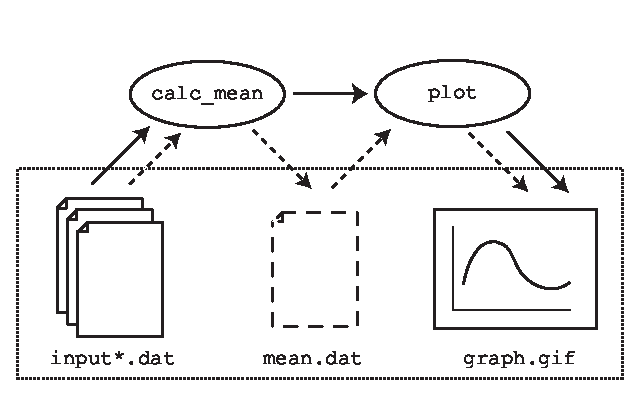
\includegraphics[height=4.2cm]{datapassing.eps}


\end{document}
